\begin{figure*}[p] % The * makes the figure span both columns, p places the figure on a float page
  \begin{center}
    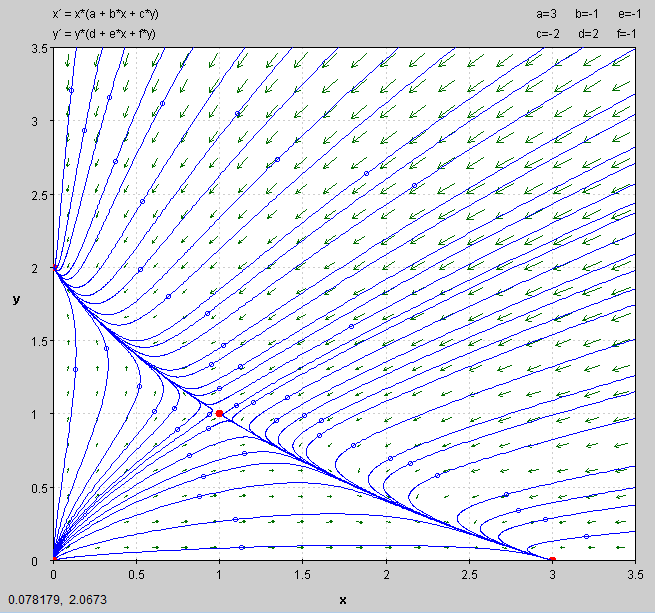
\includegraphics[width = 0.9\textwidth, height = 0.5\textwidth]{Plots/-2-1}
  \end{center}
  \caption{Phase portrait of the system in \eqref{eqn:PPSystem}, which has an unstable node at \mbox{(0,0)}, two stable points at \mbox{(0,2)} and \mbox{(3,0)} and a saddle point at \mbox{(1,1)}. All the equilibriums are marked by large dots and selected trajectories are marked by solid lines. This figure was generated using PPLANE (\texttt{http://math.rice.edu/~dfield/dfpp.html}).}
  \label{fig:pplane}
\end{figure*}

\begin{figure*}[p] % The * makes the figure span both columns, p places the figure on a float page
  \begin{center}
    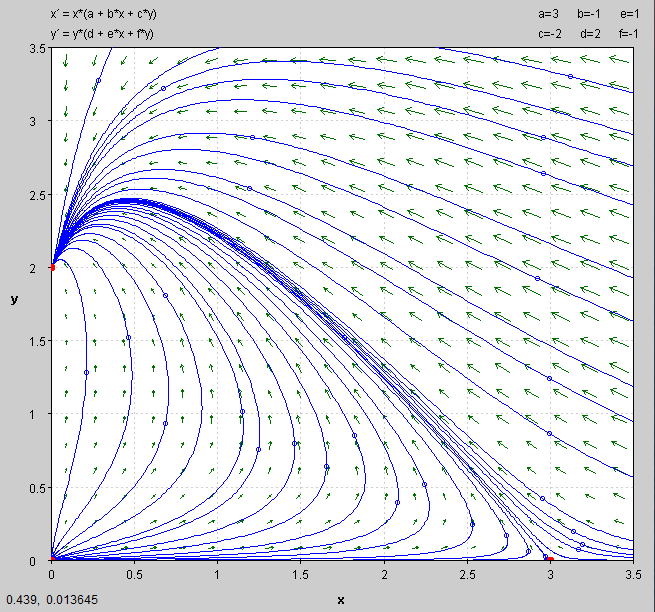
\includegraphics[width = 0.9\textwidth, height = 0.5\textwidth]{Plots/-21}
  \end{center}
  \caption{Phase portrait of the system in \eqref{eqn:PPSystem}, which has an unstable node at \mbox{(0,0)}, a stable point at \mbox{(0,2)} and a saddle at \mbox{(3,0)}. All the equilibriums are marked by large dots and selected trajectories are marked by solid lines. This figure was generated using PPLANE (\texttt{http://math.rice.edu/~dfield/dfpp.html}).}
  \label{fig:pplane2}
\end{figure*}

\begin{figure*}[p] % The * makes the figure span both columns, p places the figure on a float page
  \begin{center}
    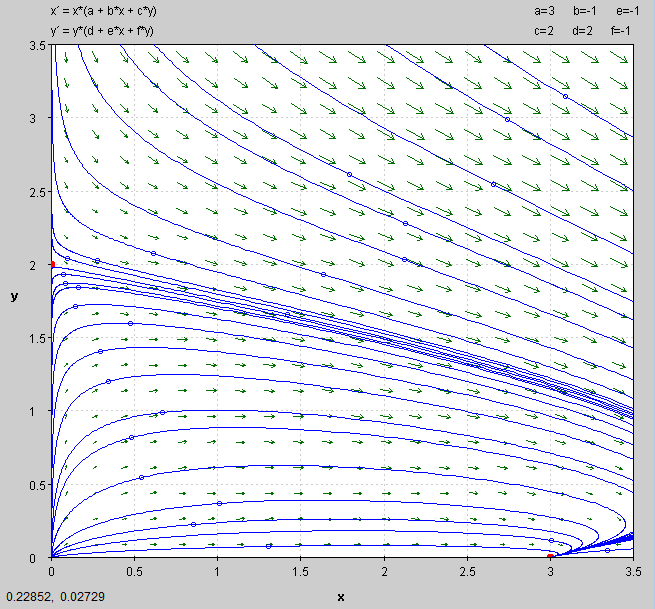
\includegraphics[width = 0.9\textwidth, height = 0.5\textwidth]{Plots/2-1}
  \end{center}
  \caption{Phase portrait of the system in \eqref{eqn:PPSystem}, which has an unstable node at \mbox{(0,0)}, a saddle point at \mbox{(0,2)} and a stable at \mbox{(3,0)}. All the equilibriums are marked by large dots and selected trajectories are marked by solid lines. This figure was generated using PPLANE (\texttt{http://math.rice.edu/~dfield/dfpp.html}).}
  \label{fig:pplane2}
\end{figure*}

\begin{figure*}[p] % The * makes the figure span both columns, p places the figure on a float page
  \begin{center}
    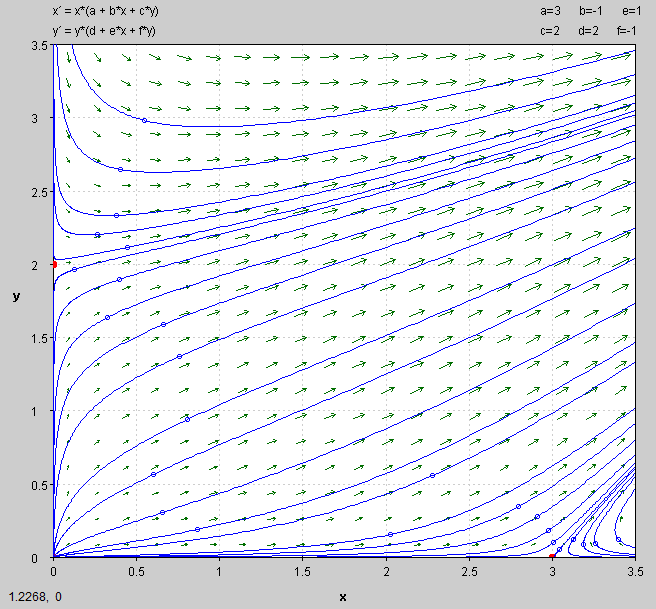
\includegraphics[width = 0.9\textwidth, height = 0.5\textwidth]{Plots/21}
  \end{center}
  \caption{Phase portrait of the system in \eqref{eqn:PPSystem}, which has an unstable node at \mbox{(0,0)}, two saddle points at \mbox{(0,2)} \mbox{(3,0)}. All the equilibriums are marked by large dots and selected trajectories are marked by solid lines. This figure was generated using PPLANE (\texttt{http://math.rice.edu/~dfield/dfpp.html}).}
  \label{fig:pplane2}
\end{figure*}

\begin{figure*}[p] % The * makes the figure span both columns, p places the figure on a float page
  \begin{center}
    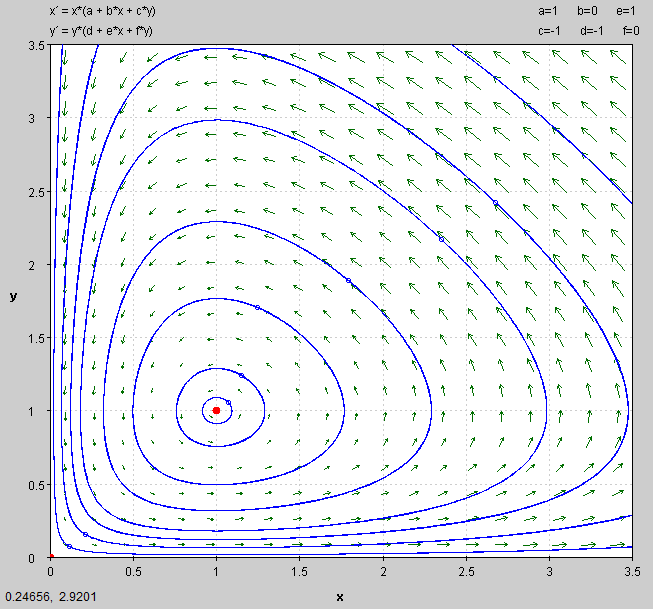
\includegraphics[width = 0.9\textwidth, height = 0.5\textwidth]{Plots/p3}
  \end{center}
  \caption{Phase portrait of the system in \eqref{eqn:PPSystem}, which has a saddle node at \mbox{(0,0)} and a stable point at \mbox{(1,1)}. All the equilibriums are marked by large dots and selected trajectories are marked by solid lines. This figure was generated using PPLANE (\texttt{http://math.rice.edu/~dfield/dfpp.html}).}
  \label{fig:pplane2}
\end{figure*}